\documentclass[a4paper,11pt]{article}
\usepackage[margin=3cm]{geometry}
\linespread{1.25}

\usepackage[T1]{fontenc}
\usepackage[utf8]{inputenc}
% \usepackage[swedish]{babel}
% \usepackage{fontspec}
% \setmainfont{Linux Libertine O}
\usepackage{lmodern}
\usepackage{graphicx}
\usepackage{float}
\usepackage{subfig}

\usepackage{fancyhdr}
\pagestyle{fancy}
\renewcommand{\headrulewidth}{ 1.0pt }
\renewcommand{\footrulewidth}{ 0.4pt }
\fancyhead{} % clear all headers
\fancyfoot{} % clear all footers

% E:even page, O:odd page, L:left, C:center, R:right
%\fancyhead[LE,RO]{\thepage}
%\fancyfoot[C]  {Albert Einstein, 2009}

\fancyhead[L]{DH2323 (DGI17) Lab 2}
\fancyhead[R]{Mikael Forsberg, Robin Gunning}
\fancyfoot[C]{\thepage}

\begin{document}
\title{\vspace{-2cm} Lab 2: Raytracing\\ \small DH2323 (DGI17)\\ KTH Royal Institute of Technology}
\author{Mikael Forsberg <miforsb@kth.se>\\ Robin Gunning <rgunning@kth.se>}
\maketitle

\vspace{-1.25cm}

\section*{Overview}
We completed all the given tasks and implemented Cramer's rule as an
optimization for the ray-triangle intersection solver.

\section*{Tracing Rays}
The instructions up to and including section 3 where quite hand-holdy (e.g copy-pastable
code for ray-triangle intersection) and the only real issue we had was caused by a
typo in checking whether or not the ray had struck the actual triangle and not just
the triangle plane (Figure 1a).

We didn't switch to using Cramer's rule for the intersection solver until much later. Some
of our experiences from implementing Cramer's rule can be found later in this document.

After locating and fixing the typo we arrived at the expected result (Figure 1b).

\begin{figure}[H]
    \centering
    \subfloat[With typo]{{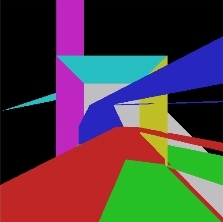
\includegraphics[width=5cm]{error.jpg} }}
    \qquad
    \subfloat[Without typo]{{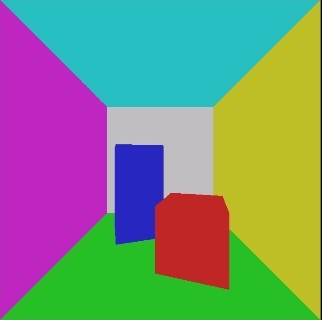
\includegraphics[width=5cm]{nolight.jpg} }}
    \caption{Tracing rays}
\end{figure}

\section*{Moving the Camera}
We initially added camera movement by simply adding or subtracting constant-valued vectors
to the camera position vector. We then consulted Wikipedia for the standard $R_y$ rotation
matrix and added controllable yaw, after which we changed our movement to adding or
subtracting the appropriate column vectors of the rotation matrix as instructed.

The fact that GLM/GLSL matrix types take arguments as column vectors as opposed to row vectors
was and still is a source of confusion. There is some kind of cognitive struggle between wanting to
set the arguments to the columns of the matrix we want (so we get the exact matrix, but it looks
wrong in the code) and accepting that if we just enter the arguments as rows we get the transpose (so
it looks right, but isn't). It is also surprisingly difficult to find material on the method of
extracting the camera heading from the row vectors (column vectors of the transpose) of the rotation matrix.

Mikael experimented with adding pitch and roll to the camera and quickly found himself looking
at YouTube videos explaining ''Gimbal Lock'' and subsequently abandoned the attempt. The idea of
trying quaternions for camera rotation came up but was never attempted.

\section*{Illumination}

We had two issues getting the initial lighting to work. The first issue
was caused by not clamping the factor involving the dot product to
a non-negative range which resulted in ''negative'' lighting manifesting
in the scene. This was resolved by reading the given formula properly
and applying the \texttt{max} function as instructed. The second issue was
caused by a bizarre typo in calculating the dot product itself (an extra
asterisk after the \texttt{n.y} term):

\begin{center}
\texttt{float dot = r.x*n.x + r.y*n.y* + r.z*n.z;}
\end{center}

\begin{figure}[H]
    \centering
    \subfloat[With typo]{{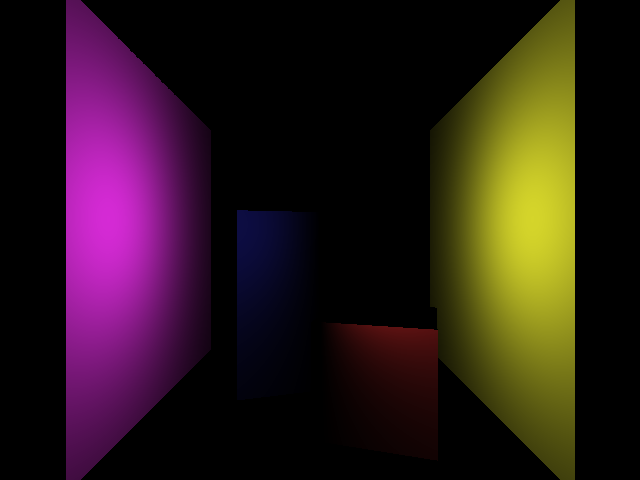
\includegraphics[width=5cm]{dotprodtypo.png} }}
    \qquad
    \subfloat[Without typo]{{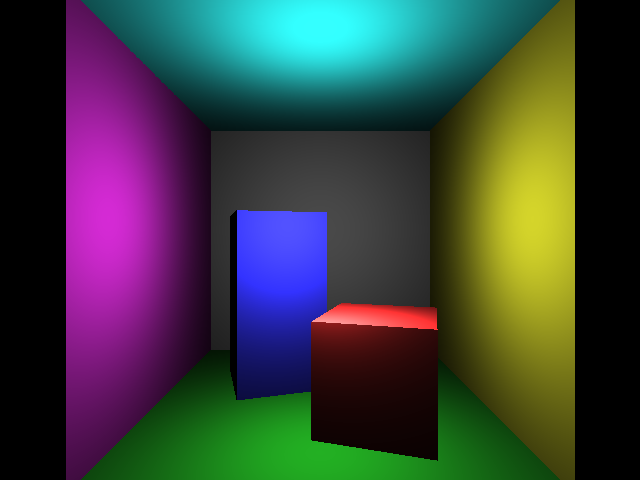
\includegraphics[width=5cm]{dotprodgood.png} }}
    \caption{Direct lighting}
\end{figure}

\section*{Shadows}
We had what is likely to be a very common issue implementing shadows: shadow test rays
that instantly intersect with the geometry from which it was to originate. A friend of
ours taking the same course ran into the same issue and Mikael has a vague recollection
of seeing an old discussion about it on KTH social. We solved the issue by moving the 
new ray ever so slightly in the intended direction before sending it off.

\begin{figure}[H]
    \centering
    \subfloat[Instant intersection]{{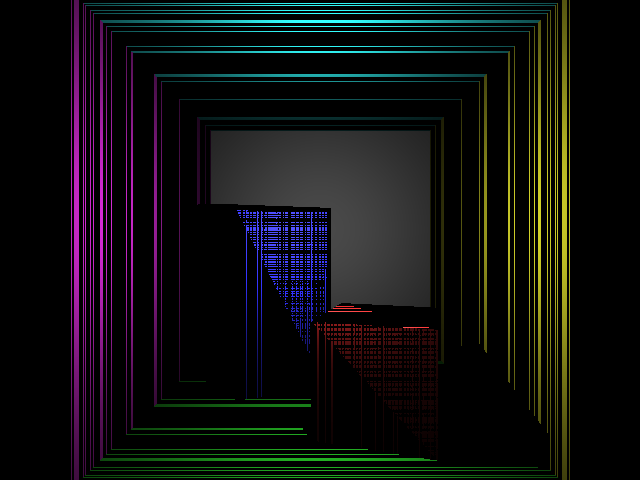
\includegraphics[width=5cm]{badshadows.png} }}
    \qquad
    \subfloat[Problem solved]{{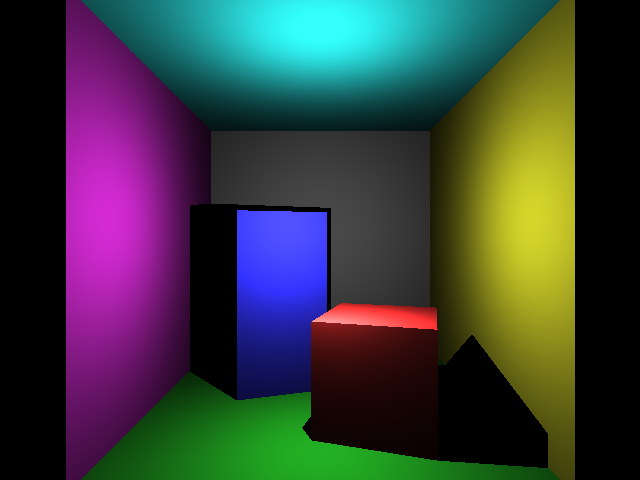
\includegraphics[width=5cm]{goodshadows.png} }}
    \caption{Shadow problems}
\end{figure}

\section*{Cramer's rule}
The main problem we experienced with implementing Cramer's rule were the myriad of
variables involved. To spare some of our sanity
we wrote down a general form of the rule (this is still in the code as a comment) and
used search-and-replace to slot in the actual variable names.

At the moment we are seeing a performance increase (in FPS) of about 32\% from using
Cramer's rule. This could probably be optimized further using some faster algorithm
for computing determinants.

\section*{Result}
Our resulting image is fairly close to the final image in the instructions document:
\begin{figure}[H]
    \centering
    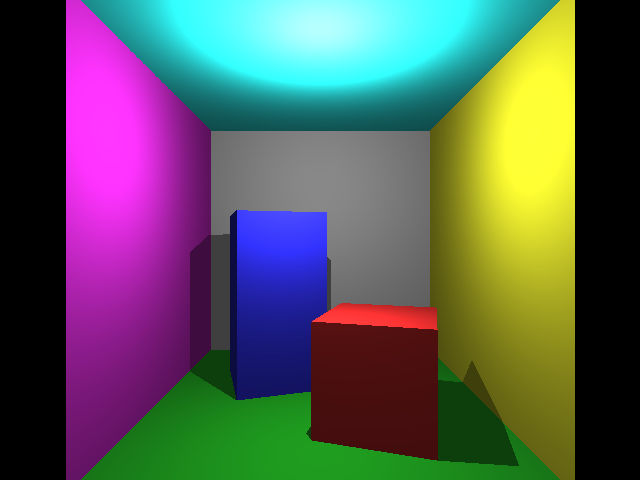
\includegraphics[width=9cm]{final.png}
    \caption{Final output}
\end{figure}

\section*{Contributions}
All tasks except for the optimization using Cramer's rule were completed as a joint effort. Mikael
implemented Cramer's rule.

\end{document}
